\documentclass{beamer}

% BIBLIOGRAPHY - BIBLATEX
\usepackage[
backend=biber,
style=apa,
bibstyle=authoryear,
citestyle=authoryear,
maxcitenames=2,
maxbibnames=99
]{biblatex}

\setlength\bibitemsep{1\itemsep} % spacing between entries in references
\addbibresource{references.bib} % .bib file


\usepackage{hyperref} %Must be loaded at the end.
\hypersetup{ %Setup of the reference links.
     colorlinks=false,
     linkcolor=black,
     citecolor=black,
     filecolor=black,
     urlcolor=black
}

\usepackage[nameinlink,capitalize]{cleveref} %For the command \cref, load after hyperref.

\usetheme{Dresden}
\title{Momentum Strategy}
\author{Digital Tools for Finance}
\date{\today}

\begin{document}

\begin{frame}
    \titlepage
\end{frame}

\begin{frame}{Outline}
    \tableofcontents
\end{frame}

\section{Introduction}
\begin{frame}{What is our project about}
    
    \begin{itemize}
        \item Momentum investing profits by buying top-performing assets and selling underperformers based on enduring price patterns. 
        \item This study examines the S\&P 500 to find the ideal lookback period for assessing past performance.
        \item Results will help managers improve risk-adjusted returns and understand momentum trends by industry.
    \end{itemize}
\end{frame}

\section{The Emergence of Momentum Strategies}


\begin{frame}{Efficient Market Hypothesis}

    \begin{itemize}
        \item The Efficient Market Hypothesis (EMH), by Eugene Fama (1970), states asset prices fully reflect all information, making consistent above-average returns unlikely.
        \item EMH has three forms: weak (prices reflect past data), semi-strong (include public info), and strong (reflect all info, including insider data).
        \item Anomalies like momentum challenge EMH, showing historical trends can predict future performance.
        \item Behavioral finance and the Adaptive Market Hypothesis suggest biases and evolving conditions make markets less efficient.
    \end{itemize}
\end{frame}


\begin{frame}{Relative Strength Strategies}
\begin{itemize}
        \item Relative Strength Strategies: Focus on ranking securities by past returns, investing in top performers, and avoiding or short-selling underperformers.
        \item Behavioral Factors: Momentum arises from market overreaction (pushing trends too far) and underreaction (delayed price adjustments).
        \item Implementation: Portfolios are built long on top-performing assets and short on underperformers, requiring regular rebalancing to adapt to trends.
        \item Risks: Momentum strategies face challenges like underperformance during market reversals, high transaction costs, and market frictions.
    \end{itemize}
\end{frame}

\begin{frame}{Cross-Sectional Momentum}
\begin{itemize}
        \item Cross-Sectional Momentum: Focuses on assets that outperform their peers, with the expectation that strong performers will continue to do well, and weak performers will stay poor (\textcite{jegadeesh1993returns}).
        \item Implementation Strategy: Involves ranking assets by historical returns, typically over 3 to 12 months, and rebalancing portfolios regularly to maintain performance (\textcite{fama1996multifactor}).
        \item Advantages: Provides diversification by including a wide range of assets and can capture excess returns from market anomalies (\textcite{moskowitz2012time}).
        \item Challenges and Risks: High transaction costs from frequent trading and vulnerability to market reversals, along with risk of overfitting historical data (\textcite{barroso2015momentum}).
    \end{itemize}
\end{frame}

\section{Methodology and Data}
\begin{frame}{Methodology and Data}
\begin{itemize}
        \item Momentum Strategies: The analysis applies long-only and long-short momentum strategies to S\&P 100 stocks, using monthly returns data from July 2014 to July 2024 to determine the ideal look-back period.
        \item Implementation: The long-only strategy selects the top 10 stocks based on historical performance, while the long-short strategy involves shorting the bottom 10 and longing the top 10, with balanced portfolio exposure.
        \item Evaluation: Sharpe ratio is used to assess risk-adjusted returns for each strategy across different look-back periods, aiming to identify the most effective momentum strategy for the S\&P 100.
    \end{itemize}
\end{frame}

\section{Findings}
\begin{frame}{Findings}
\begin{figure}
    \centering
    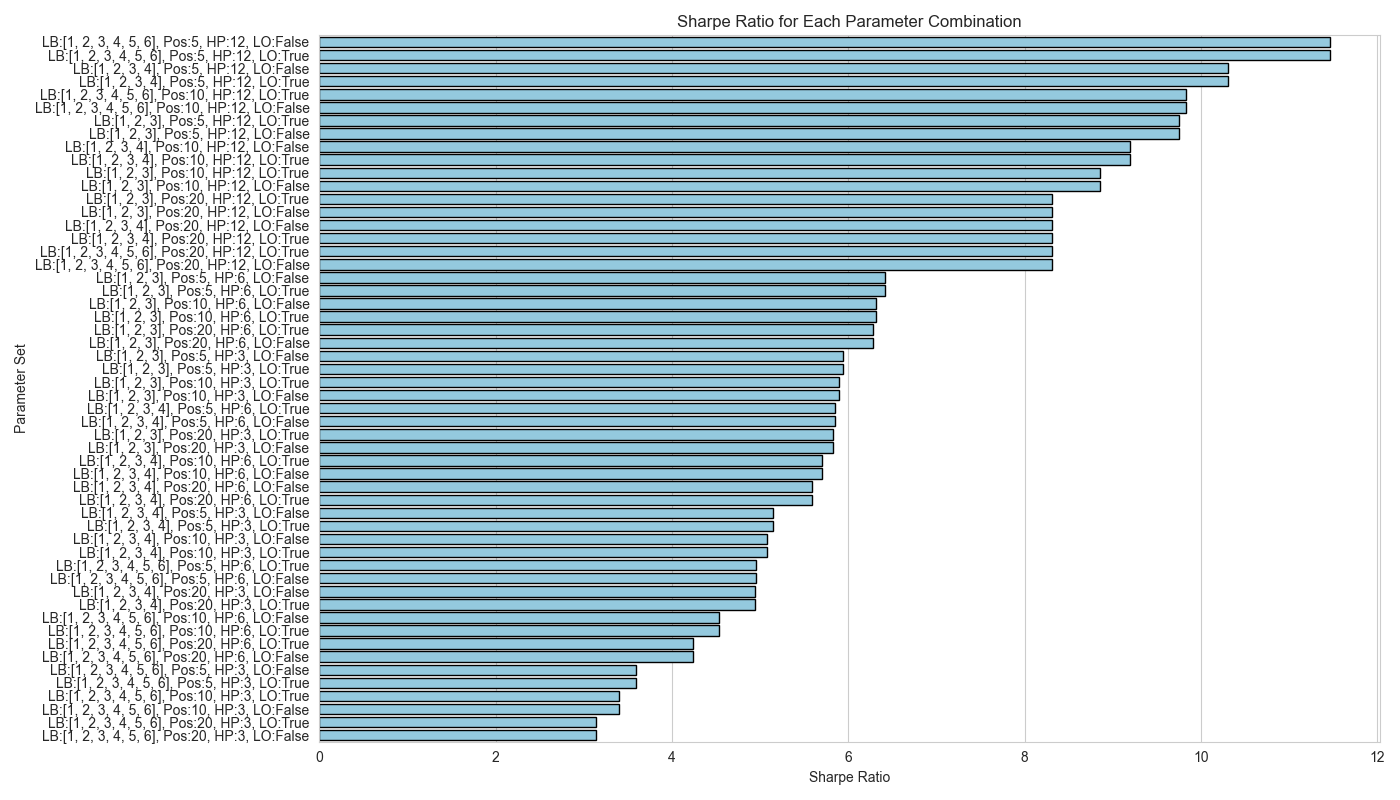
\includegraphics[width=1\linewidth]{Graphics/sharpe_ratios.png}
    \caption{Computed Sharpe Ratios}
    \label{fig:enter-label}
\end{figure}
\end{frame}

\begin{frame}{Findings}
\begin{figure}
    \centering
    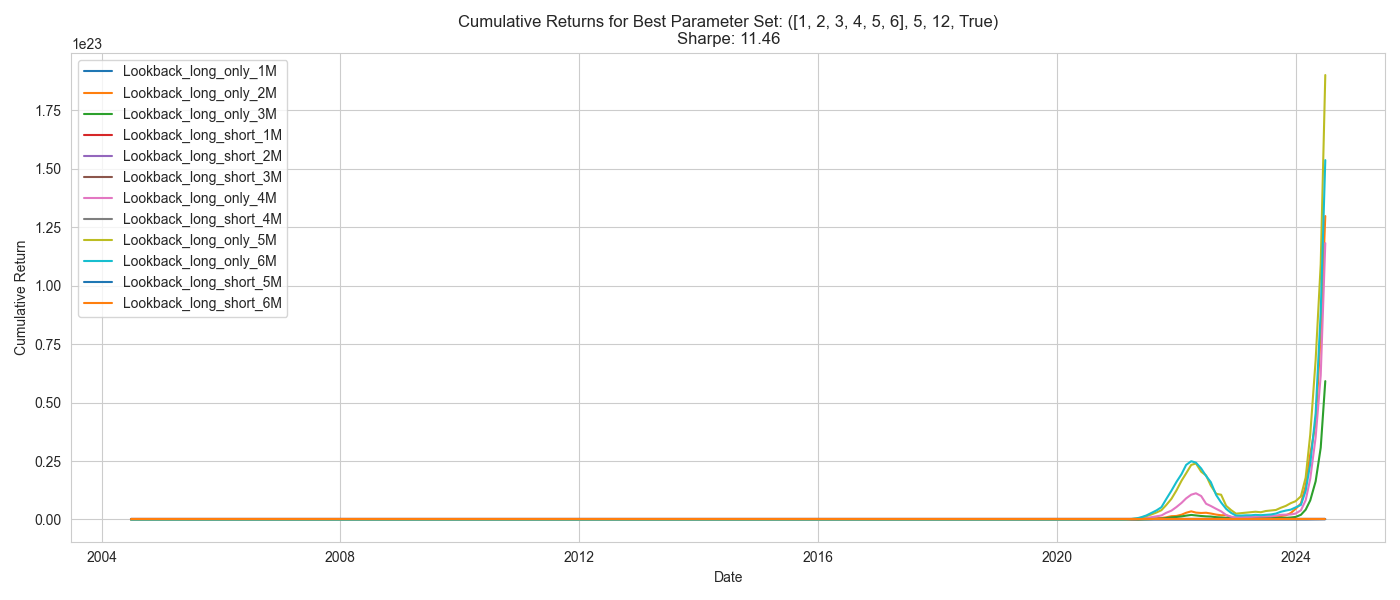
\includegraphics[width=1.05\linewidth]{Graphics/cumulative_returns_best_parameters.png}
    \caption{Cumulative Returns}
    \label{fig:enter-label}
\end{figure}
\end{frame}

\begin{frame}{Findings}
\begin{figure}
    \centering
    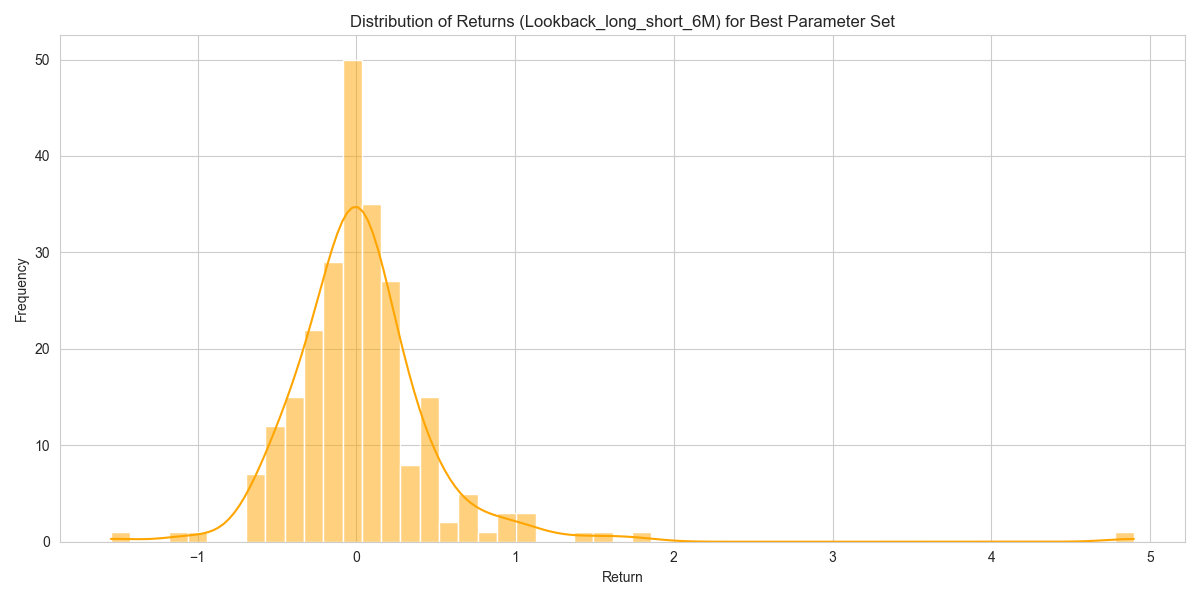
\includegraphics[width=1\linewidth]{Graphics/return_distribution.png}
    \caption{Distributed Returns}
    \label{fig:enter-label}
\end{figure}
\end{frame}

\section{Conclusion}
\begin{frame}{Conclusion}
\begin{itemize}
    \item Cumulative Returns regarding look back period of five months most profitable
    \item Returns distributed strongly around zero percent
\end{itemize}
\end{frame}


\begin{frame}{References}
    \printbibliography
\end{frame}
\end{document}